\section{Lucky Patcher} \label{section:luckypatcher-explain}
On the official website, Lucky Patcher is described as "[...] a great Android tool to remove ads, modify apps permissions, backup and restore apps, bypass premium applications license verification, and more" \cite{luckyPatcherOfficial}.
It is written by a developer called ChelpuS and currently on version is 6.0.4 (on 02/17/2016).
\newline
Lucky Patcher offers the removing of the licensing in premium apps to crack their \gls{drm}, to remove in app ads, change and restrict permissions and activities as well as to create modified after applying one of the feature above on the original \gls{apk}s \cite{luckyPatcherOfficial}.
Since copy protection by Google is deprecated, all applications are stored in \textit{/data/app/}.
The user as well as \gls{luckypatcherg} can access this folder and copy applications from it.
\textit{Root} and busybox, an application which provides standard UNIX tools for Android\cite{busyboxApp}, is only required when the application should be modified on the device, which is explained later.
\gls{luckypatcherg} requires no technical knowledge and offers automatic cracking for non professionals.
This combination makes it a popular and an effective tool with a high damage potential. \cite{munteanLicense}
\newline
This thesis focuses on how Lucky Patcher is bypassing the license verification mechanism of applications.
The goal of circumventing the license check is to make the pirated application work as if had been legally acquired in the store.
As described in section~\ref{section:lvl}, the license verification is implemented as client-server connection.
The app sends information about the user and the application to the server, which checks and verifies the given information, and replies with an approval or rejection.
The server communication is secure against man in the middle attacks or spoofing, as messages are private key encrypted \cite{munteanLicense}.
\gls{luckypatcherg} is taking a different path by modifying the application itself. This will be analysed in detail in the following chapters after explaining the general usage.
\newline
\begin{figure}[h]
    \centering
    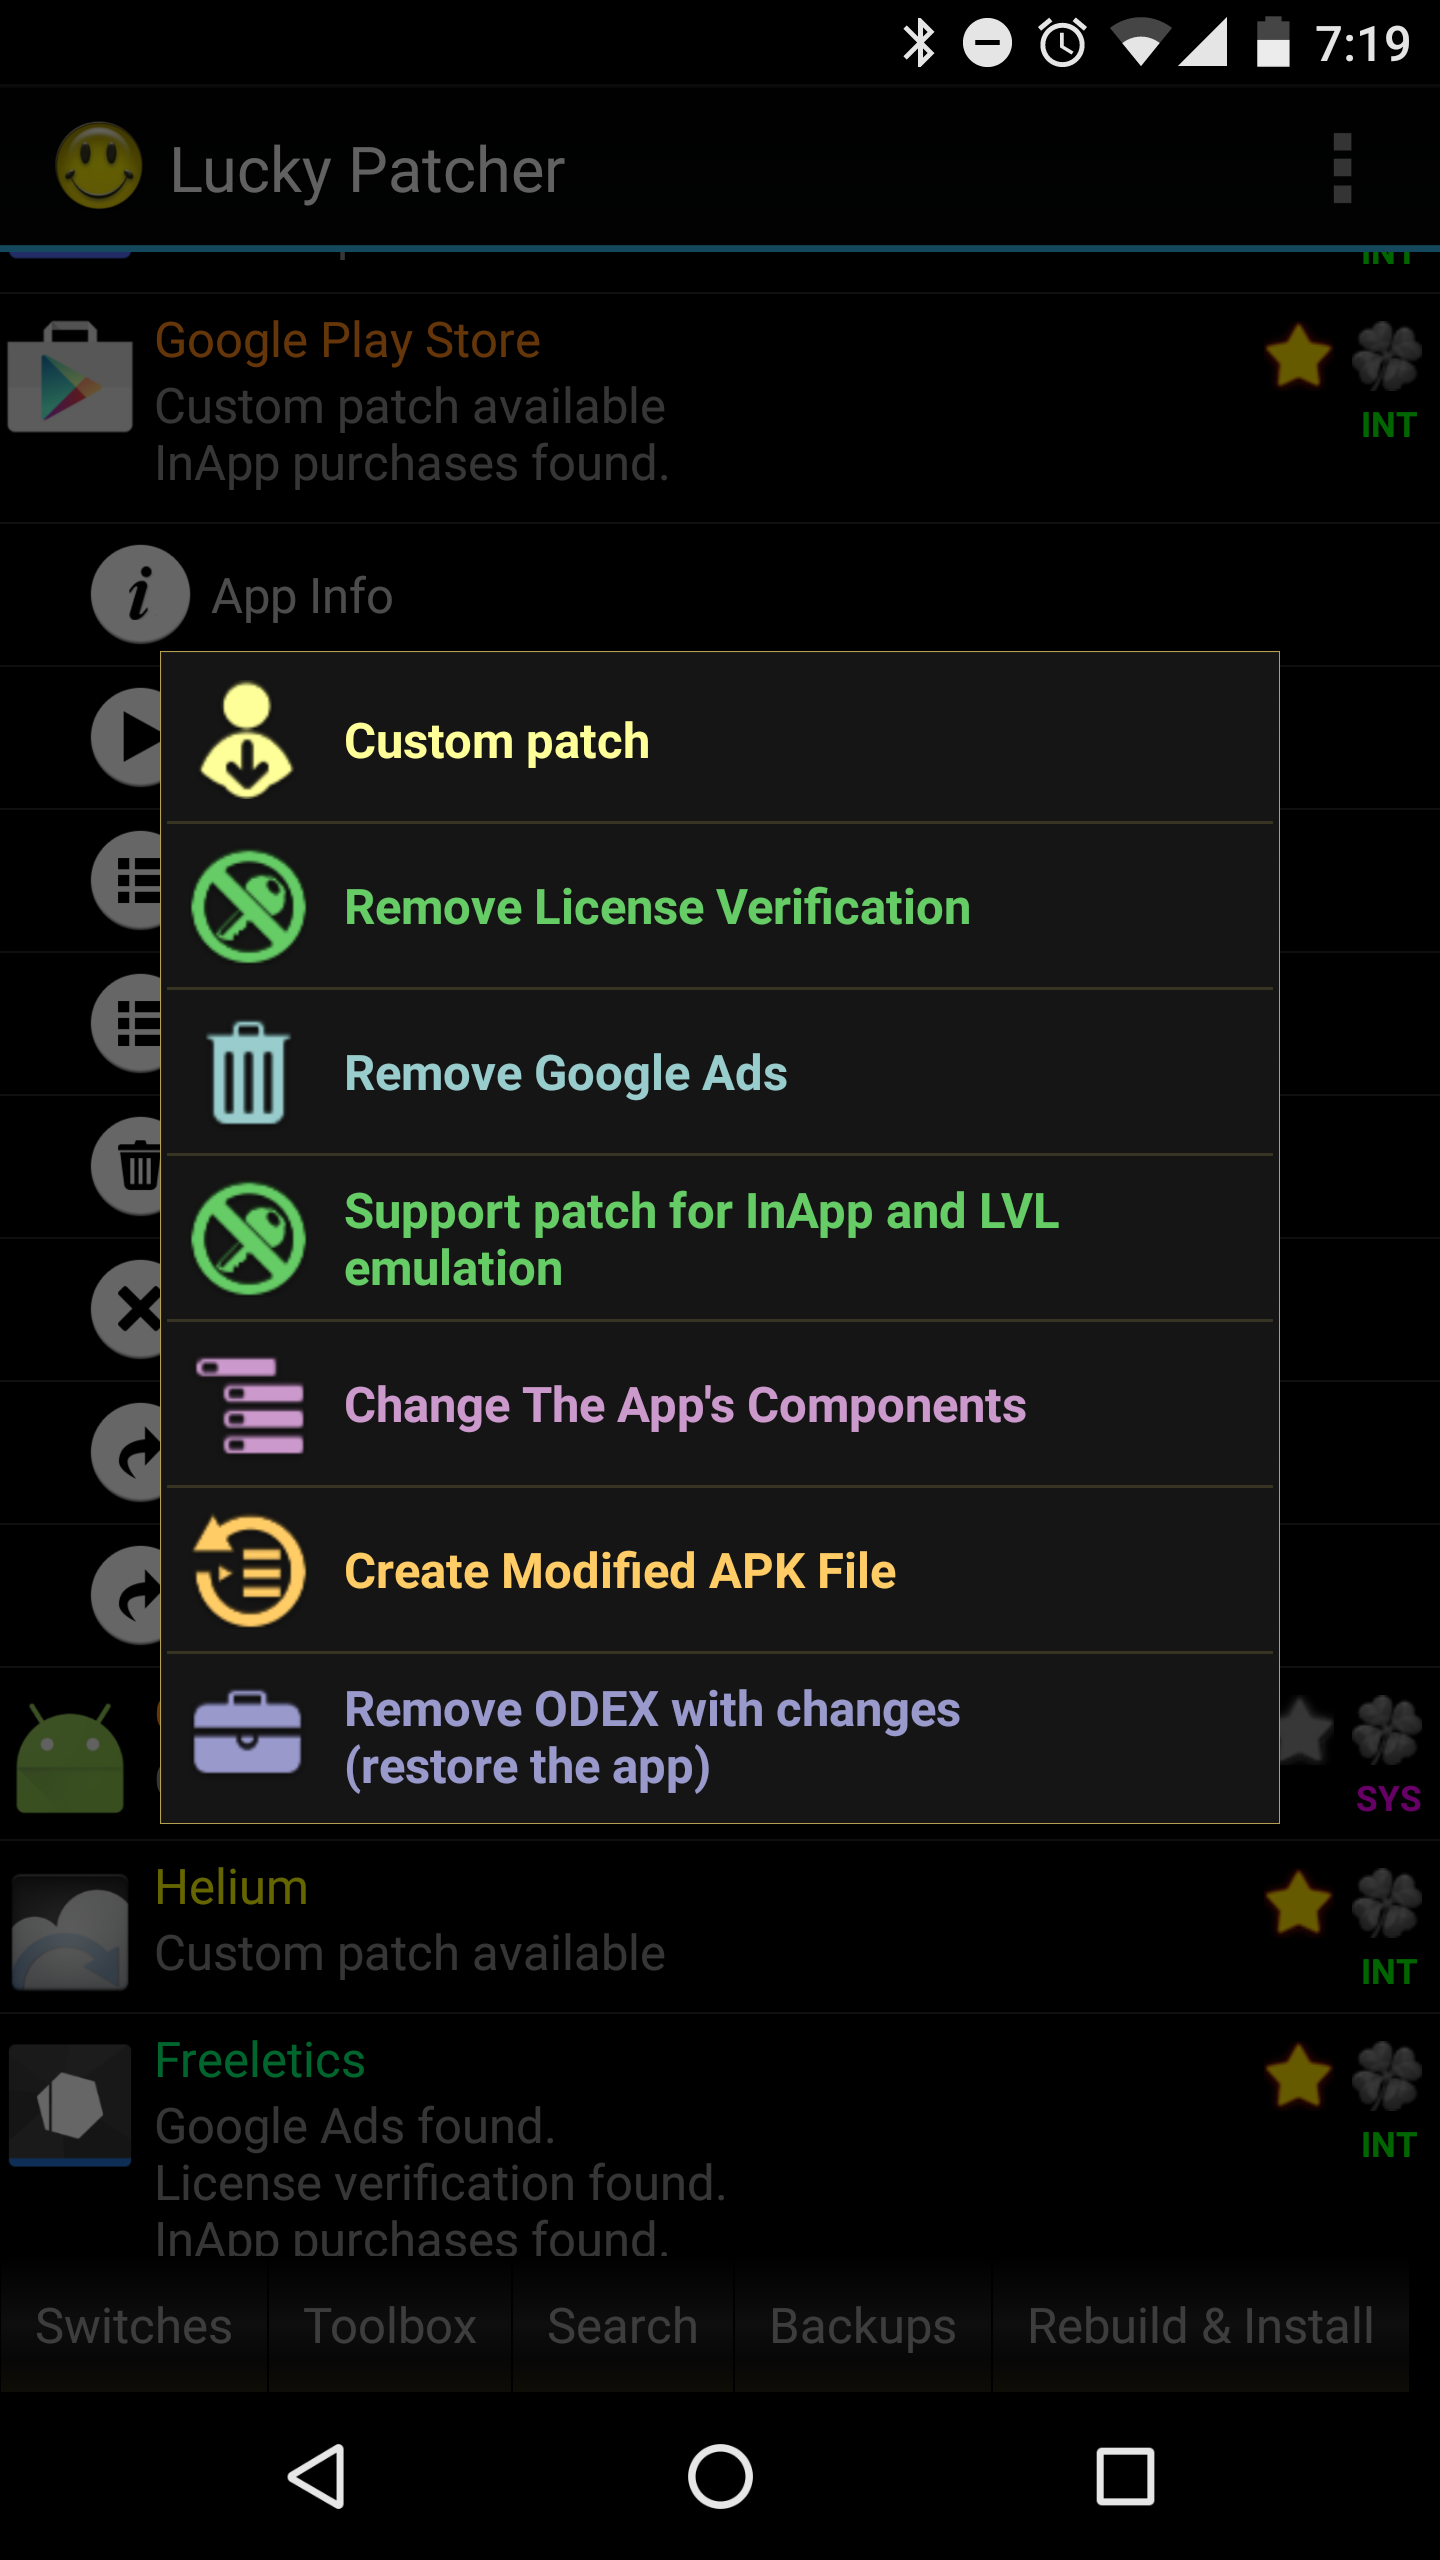
\includegraphics[width=0.3\textwidth]{data/luckyFeatures.png}
    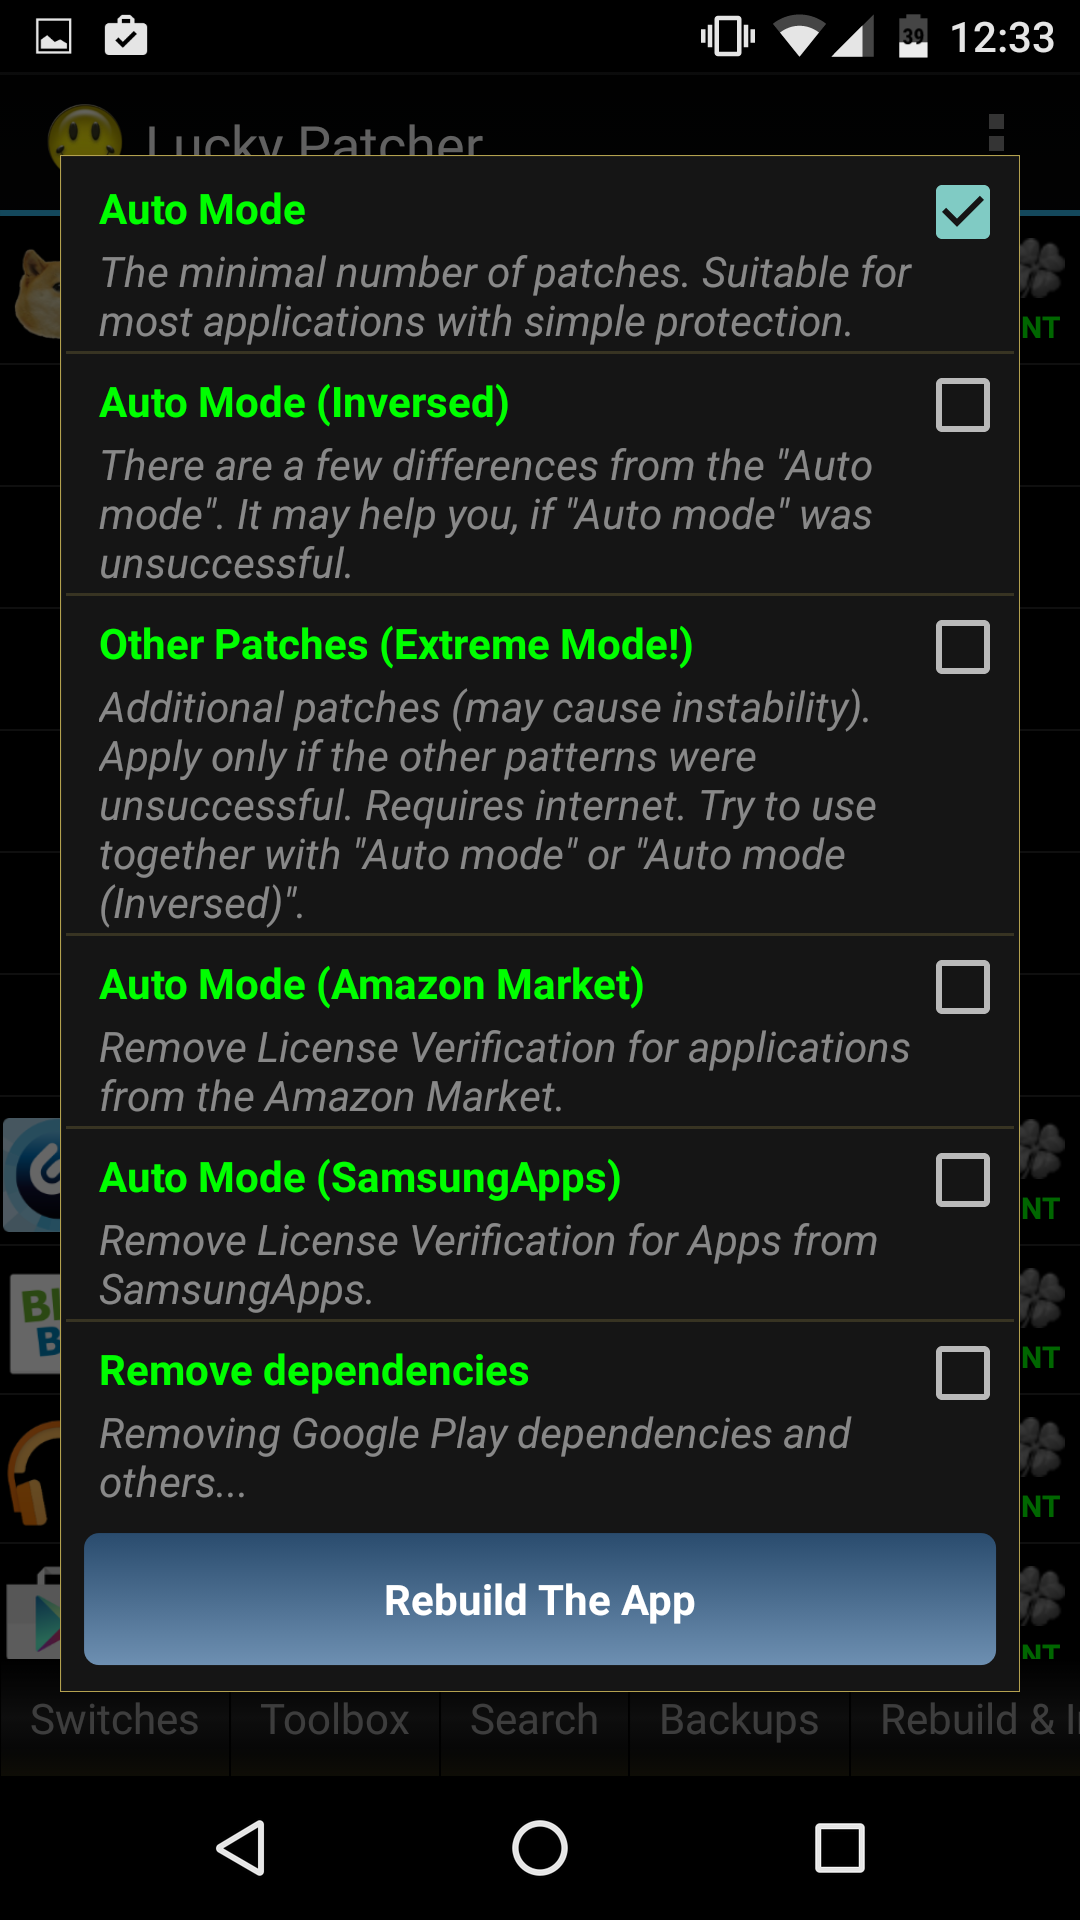
\includegraphics[width=0.3\textwidth]{data/luckyModi.png}
    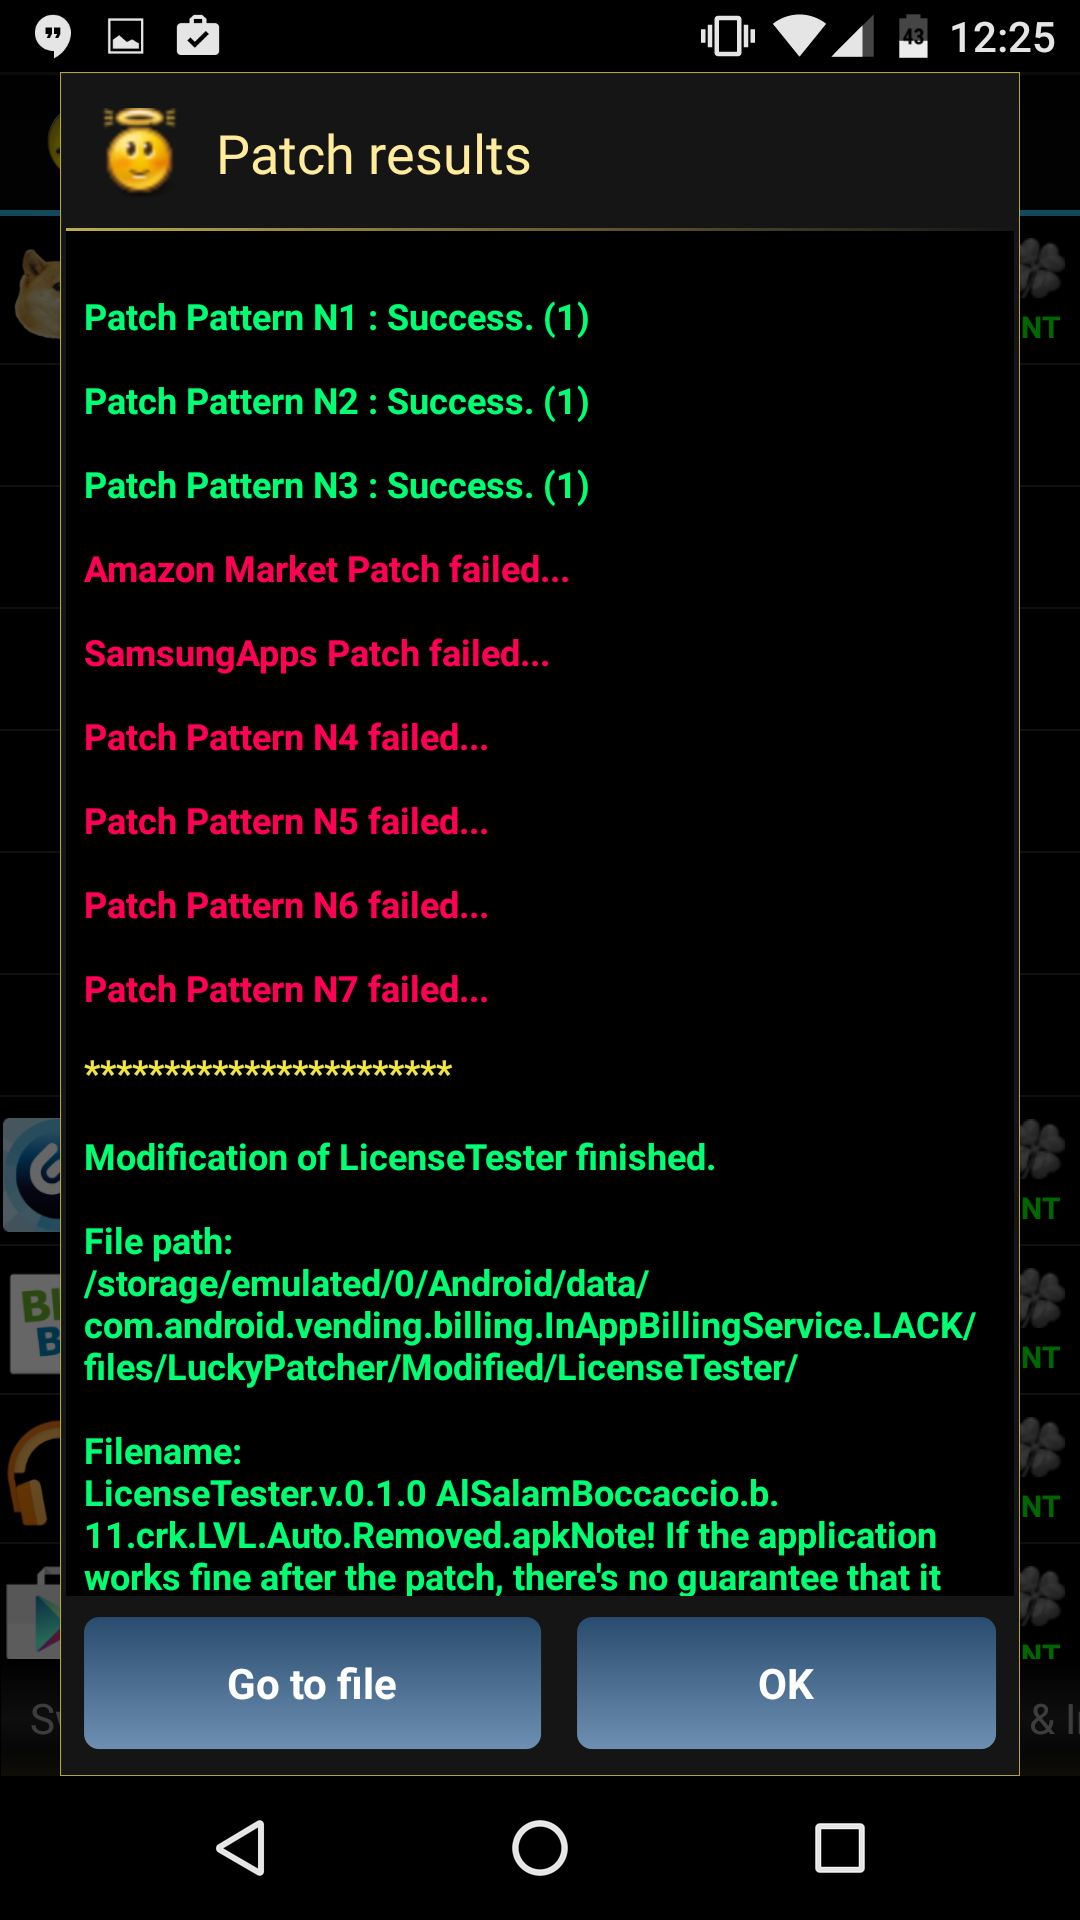
\includegraphics[width=0.3\textwidth]{data/luckyPatching.png}
    \caption{Left to right: Features offered LuckyPatcher, modes to crack license verification and the result after patching}
    \label{fig:luckyScreen}
\end{figure}

Using Lucky Patcher is fairly simple.
The application can be downloaded from the official website \cite{luckyPatcherOfficial} as an \gls{apk} and installed on the device.
In order to have the features available, the device has to be rooted.
On startup of \gls{luckypatcherg}, all installed applications are shown in a list.
An info text about what patches can be applied is shown below each name.
When a the application is selected, a submenu offers various actions, e.g. to get information about the app or run it.
Figure~\ref{fig:luckyScreen} shows the menu of patches which can be applied to the application.
These patches can either be applied in two ways.
Choice one is by applying the patch directly on the device and should be taken when \textit{root} is available.
This method creates an \gls{odex} in the Dalvik cache on the phone.
Choice two is by creating a modified \gls{apk}, which does not require \textit{root}.
In order to to run the cracked application, the original \gls{apk} has to be removed and replaced by the modified one.
Upon selecting one of the two choices for removing the license verification, different patching modes can be selected as seen in figure~\ref{fig:luckyScreen} in the middle.
Their description is rather short and does not offer information of how the modes are working.
After selecting the mode, the patching is done and the result is shown.
As seen in figure~\ref{fig:luckyScreen} on the right, different patching patterns are applied when removing license verification.
The different patching patterns are analysed and explained in section~\ref{section:luckypatcher-patterns}.
Lucky Patcher does guarantee that the result is working and all license verification related restrictions are removed.
\newline
In this thesis, Lucky Patcher is analysed in two different ways.
\begin{itemize}
\item source code reengineering
\item analysis of cracked applications and comparison with the original
\end{itemize}
